\documentclass[]{tufte-handout}

\title{Spaced Repetition}

\date{10 January 2019} % without \date command, current date is supplied

%\geometry{showframe} % display margins for debugging page layout

\usepackage{graphicx} % allow embedded images
  \setkeys{Gin}{width=\linewidth,totalheight=\textheight,keepaspectratio}
  \graphicspath{{graphics/}} % set of paths to search for images
\usepackage{amsmath}  % extended mathematics
\usepackage{booktabs} % book-quality tables
\usepackage{units}    % non-stacked fractions and better unit spacing
\usepackage{multicol} % multiple column layout facilities
\usepackage{lipsum}   % filler text
\usepackage{fancyvrb} % extended verbatim environments
  \fvset{fontsize=\normalsize}% default font size for fancy-verbatim environments

\usepackage{fontspec}
% \setmainfont[Mapping=tex-text,Numbers=OldStyle]{Bembo Book MT Std}
\setmainfont[Mapping=tex-text,Numbers=OldStyle]{Minion Pro}
\setsansfont[Mapping=tex-text,Numbers=OldStyle,Scale=MatchLowercase]{Gill Sans}
\setmonofont[Mapping=tex-text,Scale=MatchLowercase]{Operator Mono}
% Set up the spacing using fontspec features
\renewcommand\allcapsspacing[1]{{\addfontfeature{LetterSpace=15}#1}}
\renewcommand\smallcapsspacing[1]{{\addfontfeature{LetterSpace=10}#1}}

% Standardize command font styles and environments
\newcommand{\doccmd}[1]{\texttt{\textbackslash#1}}% command name -- adds backslash automatically
\newcommand{\docopt}[1]{\ensuremath{\langle}\textrm{\textit{#1}}\ensuremath{\rangle}}% optional command argument
\newcommand{\docarg}[1]{\textrm{\textit{#1}}}% (required) command argument
\newcommand{\docenv}[1]{\textsf{#1}}% environment name
\newcommand{\docpkg}[1]{\texttt{#1}}% package name
\newcommand{\doccls}[1]{\texttt{#1}}% document class name
\newcommand{\docclsopt}[1]{\texttt{#1}}% document class option name
\newenvironment{docspec}{\begin{quote}\noindent}{\end{quote}}% command specification environment

\usepackage{multicol}

\usepackage{enumitem}
\setlist{nosep} % or \setlist{noitemsep} to leave space around whole list

\begin{document}

\maketitle% this prints the handout title, author, and date

\marginnote{Ben Deaton \\ \noindent\url{http://jbendeaton.com}}

\begin{abstract}
\noindent
This document describes how to use spaced repetition to efficiently memorize information. I cover my motivation for exploring this, the science of spaced repetition, tools you can use to implement a spaced repetition memory system, and best practices for card creation and review.
\end{abstract}


\section{Why?}

\begin{itemize}
	\item Currently trying to quickly ramp/expand knowledge in two fields:
	\begin{itemize}
		\item Computational genomics because daughter's rare genetic disorder
		\item Machine learning for career in general (books, MOOCs)
	\end{itemize}
	\item Frequently feel like I don't retain enough of what I read
	\item Then, I saw Michael Nielsen\footnote{Quantum physicist, author, and computer scientist \url{https://en.wikipedia.org/wiki/Michael_Nielsen}} post a tweetstorm\cite{nielsen_twitter} about spaced repetition and all the ways he uses it. He goes on for 50 tweets and it gets better and better:

\begin{figure}
  \hspace{1cm} 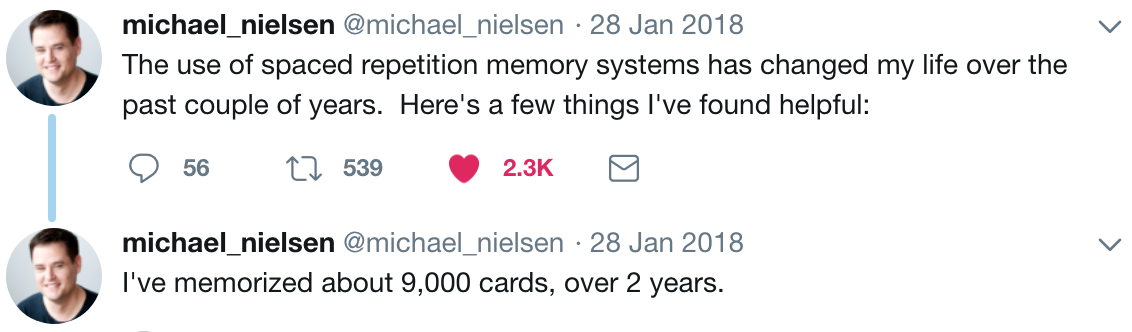
\includegraphics[width=0.7\linewidth]{nielsen_twitter.png}
  \caption{Wat? 9000 cards wtf?}
  \label{fig:twitter}
  \setfloatalignment{c}
\end{figure}

	\item Nielsen went on to write an essay\cite{nielsen} about his experience using a spaced repetition memory application called Anki\footnote{Anki is the Japanese word for ``memorization''}.
\end{itemize}

\subsection{So, like, flash cards?}

Yes.

\subsection{The Promise of Spaced Repetition}
\begin{itemize}
	\item Make the things you remember a conscious \textit{choice} (do not leave to \textit{chance})
	\item Exploit memory research to learn with extreme efficiency\footnote{Robert Craig set multiple records on the quiz show Jeopardy! 2010-2011 in part thanks to using Anki to memorize chunks of a collection of >200,000 past questions.}
	\item Lifetime effort per fact/card < 5 minutes
\end{itemize}

\subsection{Possible Topics to Memorize}

\begin{fullwidth}

\begin{multicols}{4}
\begin{itemize}
    \item Quotes
    \item Vocabulary
    \item Foreign language
    \item Historical events
    \item Industry jargon
    \item Computer commands
    \item Demographic statistics
    \item Facts about cities
    \item Frequent mispellings
    \item Political figures
    \item Best dish at restaurant
    \item Programming language syntax
    \item Unit conversions
    \item Trivia about people
    \item Philosophical concepts
    \item Logical fallacies
    \item Study material
    \item Paintings or artists
    \item Recipes
    \item How to exit \texttt{vim} :)
    \item Anything you look up repeatedly
    \item Anything you're embarrassed you don't know
    \item ?
\end{itemize}
\end{multicols}

\end{fullwidth}

\section{Science of Spaced Repetition}

Gwern Branwen has compiled probably the definitive online resource\cite{gwern} on the science of memory\footnote{Much of this research has been replicated!}. Here is a brief summary:

\begin{figure}[h]
  \hspace{1cm}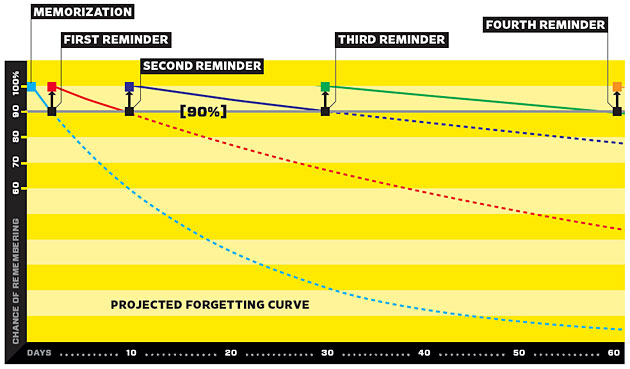
\includegraphics[width=0.8\linewidth]{forgetting-curve-wired-wozniak.jpg}
  \caption{Forgetting Curve with Retest (Slopes are exaggerated to illustrate the concept. The initial decay is actually much steeper per Figure \ref{fig:ebbinghause})}%
  \setfloatalignment{c}
\end{figure}

\begin{itemize}
	\item The ``Forgetting Curve'': Memory decays exponentially (like radioactive half-life). Ebbinghause (1885) memorized a series of nonsense syllables and retested at periods ranging from 20 minutes to 31 days. See Figure \ref{fig:ebbinghause}.

\begin{marginfigure}%
  \fbox{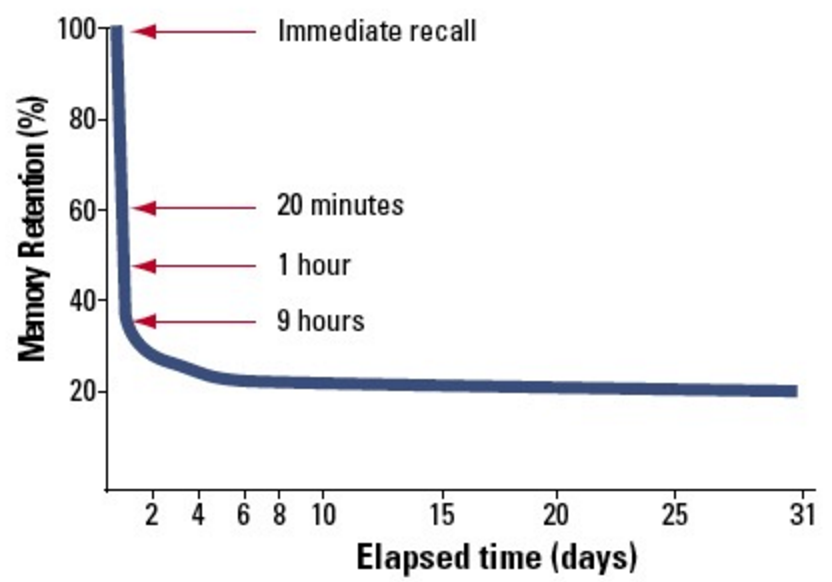
\includegraphics[width=0.75\linewidth]{stahl-cropped.png}}
  \caption{Ebbinghaus (1885) Forgetting Curve (Steep!)}
  \label{fig:ebbinghause}
\end{marginfigure}

\begin{marginfigure}%
  \fbox{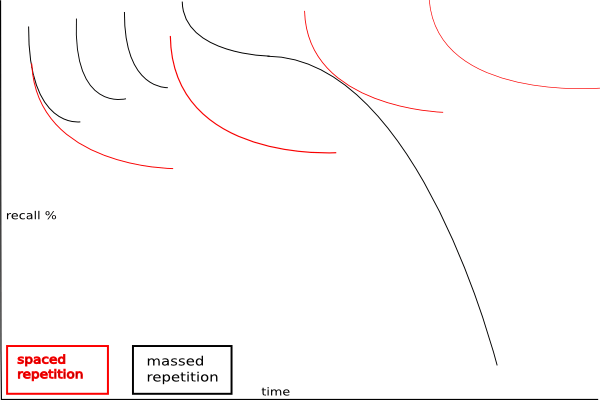
\includegraphics[width=0.75\linewidth]{forgetting-curves.png}}
  \caption{Cramming (black) vs. Spaced Repetition (red)}
  \label{fig:cramming}
\end{marginfigure}

	\item Initial rate of decay varies based on complexity of information, similarity to other things you know, and other unknown factors
	\item Review resets probability of recall (you go back to 1.0)
	\item Rate of decay decreases after retest
	\item Change in rate of decay seems to be function of elapsed time between retest (how much decay occurs before retest)
	\item Decay following cramming is roughly equivalent to or slightly better than learning once with no review. See Figure \ref{fig:cramming}.
	\item Spaced repetition systems exploit these properties of memory to efficiently retest at the most optimal time for reinforcement and slowing of recall decay.

\end{itemize}

\section{Available Tools that use Spaced Repetition}

\begin{itemize}
	\item Anki\cite{anki}
	\begin{itemize}
		\item Very popular, extensible, open source
		\item Available and syncs across web, desktop (Mac/Windows), mobile (iOS/Android) clients
		\item Types of cards available:
		\begin{itemize}
			\item Basic question and answer (front and back)
			\item Basic with reversed (front-back and back-front)
			\item Basic but type in the answer first
			\item Cloze deletion (fill-in-the-blank)
		\end{itemize}
		\item Can use text, graphics, audio, and \LaTeX equations as question or answer
	\end{itemize}
	\item Others: Mnemosyne, SuperMemo, Brainscape
\end{itemize}

\section{Process}

\begin{itemize}
	\item Start-up and Mindset

	\begin{itemize}
		\item Install Anki on desktop and mobile and get sync working.
		\item Train yourself that you now have a bucket where information goes that you want to remember.
		\item Treat Anki as a tool that sits alongside your reading/learning process.
	\end{itemize}

	\item Create cards
	\begin{itemize}
		\item Create your own cards instead of downloading pre-made decks
		\item Start small. Don't overwhelm yourself by creating 200 cards at first.
		\item Either create cards as you read, or develop a system for adding them later (i.e. write a boxed A\marginnote{\fbox{A}} in the margin as you read a book, email links to yourself with the data you want to Ankify, etc.)
		\item Consensus: Create in desktop app, review in mobile app
		\item See best practices below for card creation
	\end{itemize}

	\item Review/Study
	\begin{itemize}
		\item Does not require huge chunks of time\footnote{Nielsen learned 9000 cards in < 20 min per day.}
		\item Exploit small windows of downtime (standing in line, on hold, waiting for kettle to boil, other indisposed moments)\marginnote{Pro tip: Replace mindless social media scrolling with Anki}
		\item Stages of Learning in Anki:
		\begin{itemize}
			\item New: Card just created. You haven't seen it yet in an Anki session.
			\item Learning: Again (<1 minute), Good (<10 minutes), and Easy (4d). Once you hit Easy, the ard moves into the Review stage.
			\item Review: Rating recall as Good will increase the review duration by 2.5x\footnote{At rate of growth of 2.5x per successful recall, cards rapidly reach a review frequency of many months.}. Rating as Hard or Easy will shorten or lengthen the review duration. Anki will detect cards that are Lapsing (forget a card you already learned and it moves back into Learning) and Leeches (cards that you repeatedly Lapse on). Leeches are too hard or poorly designed.
		\end{itemize}
		\item Configure the number of new and review cards per day\footnote{Defaults are 20 new and 100 review.}
		\item The iOS Review Mode is shown in Figure \ref{fig:review}.

\begin{figure}
  \hspace{1cm}\fbox{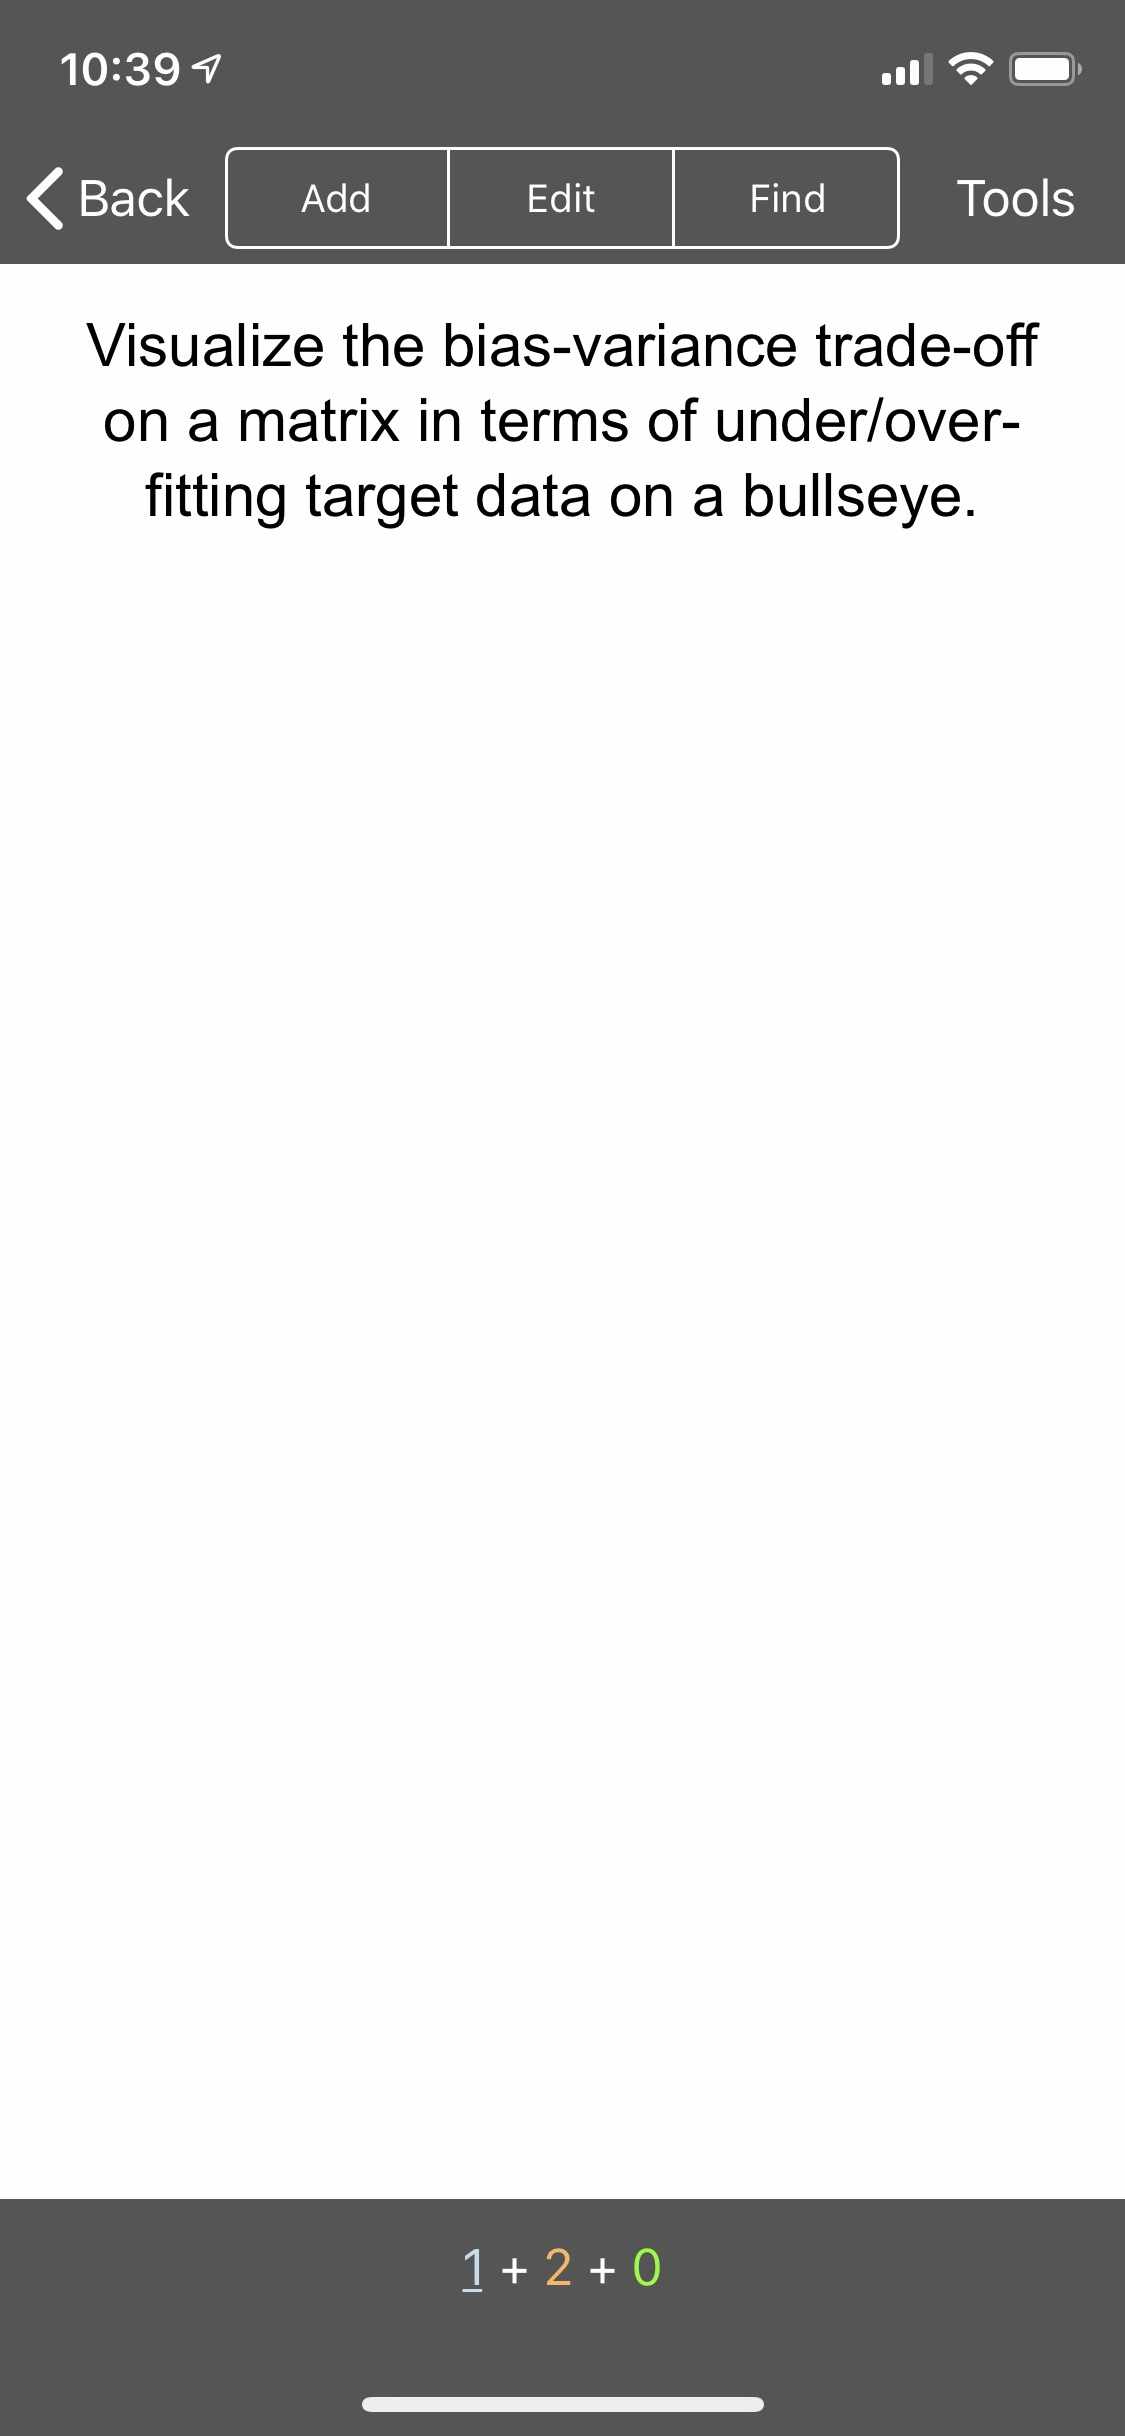
\includegraphics[width=0.3\linewidth]{IMG_9803.jpg}}
  \hspace{1cm}\fbox{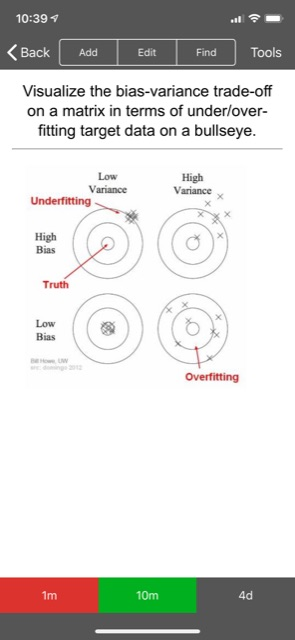
\includegraphics[width=0.3\linewidth]{IMG_9804.jpg}}
  \caption{Anki Review Mode}
  \label{fig:review}
  \setfloatalignment{c}
\end{figure}

	\end{itemize}
\end{itemize}




\section{Best Practices}


\subsection{Anki Essentials, by Alex Vermeer}

Alex Vermeer wrote a short e-book called Anki Essentials\cite{vermeer} which is an excellent introduction to the mechanics of Anki. It walks you through setup of a sample deck, your first review of that deck, and then deep dives into power user tooling. I highly recommend this resource and think it will save you a lot of time getting up to speed. It's only \$5.

\newpage

\subsection{Augmenting Longterm Memory, by Michael Nielsen}

To really get into the mind of a master on this topic, Michael Nielsen\cite{nielsen} also published an essay on this topic after his Twitter thread generated so much response. This paper is a fun look into a brilliant scientist's process.

In this article, he does a deep dive on his process for using Anki. He describes how to use Anki to thoroughly read a research paper in an unfamiliar field\footnote{Which is how he wrote this article: \url{https://www.quantamagazine.org/is-alphago-really-such-a-big-deal-20160329/}}, using Anki to do shallow reads of papers, how he uses Anki to memorize the meaning of technical graphs, and syntopic reading of unfamiliar fields (grokking the overall view of an entire field).

A few patterns of advice or topics from Nielsen that overlap slightly with Wozniak's advice below:

\begin{itemize}
	\item Make most Anki questions and answers as atomic as possible
	\item Anki use is best thought of as a virtuoso skill, to be developed
	\item Anki isn't just a tool for memorizing simple facts. It's a tool for understanding almost anything.
	\item Use one big deck
	\item Avoid orphan questions (they are probably irrelevant)
	\item Don't share decks / Construct your own decks
	\item Cultivate strategies for elaborative encoding / forming rich associations (represent the same information multiple ways)
	\item Challenges of using Anki to store facts about friends and family (Most appreciate the effort although it may come across as strange if they know you do it)
	\item 95\% of Anki's value comes from 5\% of the features (I.e. no need to go crazy)
	\item Procedural versus declarative memory (use what you learn)
	\item Get past ``names don't matter'' and don't take Feynman\footnote{``I learned very early the difference between knowing the name of something and knowing something.'' Richard Feynman} too far. Learning art is a great use-case.
	\item What do you do when you get behind? Catching up is not as bad as you think it will be.
	\item Using Anki for APIs, books, videos, seminars, conversations, the web, events, and places
	\item Avoid the yes/no pattern
	\item And more!
\end{itemize}



\subsection{Wozniak's Rules of Formulating Knowledge\cite{wozniak}}

\begin{enumerate}
\item{Do not learn if you do not understand}

\begin{quote}
Richard Feynman, in the essay \textit{O Americano, Outra Vez!}, relates the analogy of a Greek scholar who comes to a new country to find everyone studying Greek, even small kids in elementary schools\footnote{In the book: Richard P. Feynman. \textit{Surely You’re Joking Mr. Feynman!}, 1985.}:

\begin{quote}
The Greek scholar goes to the examination of a student who is coming to get his degree in Greek, and asks him, ``What were Socrates' ideas on the relationship bewteen Truth and Beauty?''--and the student can't answer. Then he asks the student, ``What did Socrates say to Plato in the Third Symposium?'' the student lights up and goes ``Brrrrrrrrr-up''--he tells you everything, word for word, that Socrates said, in beautiful Greek.

But what Socrates was talking about in the Third Symposium was the relationship bewteen Truth and Beauty!
\end{quote}
\end{quote}

\item{Learn before you memorize}
\begin{quote}
To drastically reduce learning time, start by obtaining an understanding of the big picture or overall structure of the topic you are trying to learn. Then, you have a container in which to place narrower facts. Go for breadth, then depth. Do not start memorizing loosely-relatd facts about a topic.
\end{quote}

\item{Build upon the basics}

\begin{quote}
Start with the most simple and seemingly obvious things and gradually build complexity off of them.
\end{quote}

\item{Stick to the minimum information principle}

\begin{quote}
Formulate material into the simplest form possible to make it (a) easier to remember and (b) spaced review easier to schedule. Answers should be as short as possible.

Bad (1 question): What are the characteristics of the Dead Sea?

Good (9 questions): Where is the Dead Sea located? What is the lowest point on the Earth's surface? What is the average level on which the Dead Sea is located? How long is the Dead Sea? How much saltier is the Dead Sea than the oceans? What is the volume content of salt in the Dead Sea? Why can the Dead Sea keep swimmers afloat? Why is the Dead Sea called Dead? Why only simple organisms can live in the Dead Sea?
\end{quote}

\item{Cloze deletion is easy and effective}

\begin{quote}
Omitting words or phrases (fill-in-the-blank) helps greatly in sticking to the minimum information principle.

Example: $\rule{1cm}{0.15mm}$ deletion is easy and effective.
\end{quote}

\item{Use imagery}

\begin{quote}
Instead of ``What is the law of supply and demand in words?'', ask ``Explain the law of supply and demand visually'' and see if you can draw the figure (set the figure as the card's answer).

\begin{marginfigure}%
  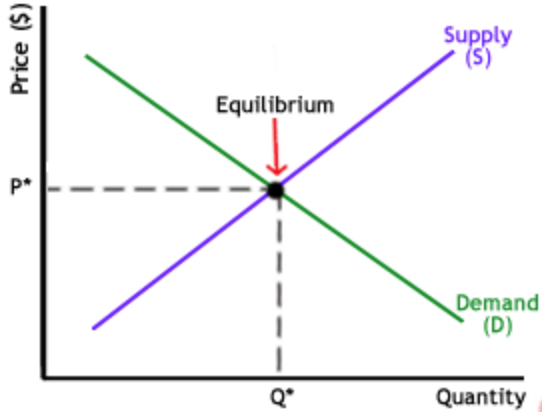
\includegraphics[width=0.7\linewidth]{supply-demand.png}
  % \caption{\url{https://twitter.com/michael_nielsen/status/957763229454774272}}
  % \label{fig:twitter}
\end{marginfigure}

Think of creative ways to use photographs, figures, maps, diagrams, or art to reinforce concepts you are trying to learn.
\end{quote}

\item{Use mnemonic techniques}

\begin{quote}
A mnemonic is a general term for a tool or trick that aids information retention. Apparently Tony Buzan is resource for mnemonic techniques.
\end{quote}

\item{Graphic deletion is as good as cloze deletion}

\begin{quote}
Graphic deletion is exactly the same as cloze deletion except it omits portions of images rather than sentences. Graphic deletion is great for learning things like anatomy, geography, or labels on other types of diagrams.

\begin{marginfigure}%
  \fbox{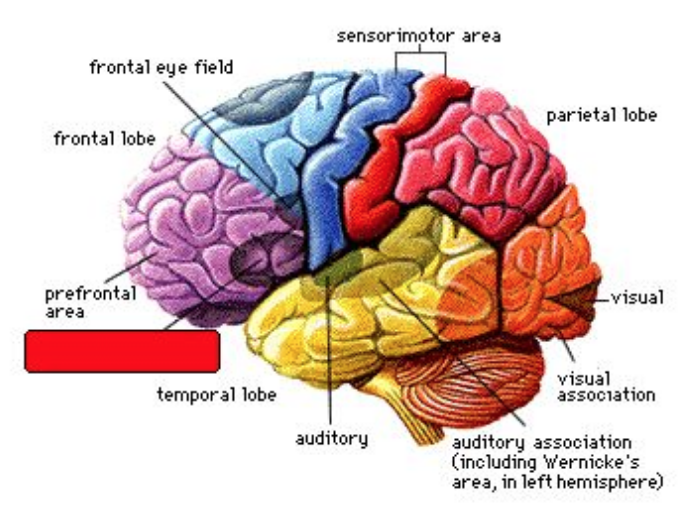
\includegraphics[width=0.7\linewidth]{graphic-deletion.png}}
  % \caption{\url{https://twitter.com/michael_nielsen/status/957763229454774272}}
  % \label{fig:twitter}
\end{marginfigure}

\end{quote}

\item{Avoid sets}

\begin{quote}
Sets are collections of objects and are very hard to remember. They are also inefficient to memorize because they are prone to all-or-nothing evaluation.

Avoid questions like ``What are all the countries in the EU?'' and instead ask questions around associating facts between the EU and specific countries or a small subset of related countries.
\end{quote}

\item{Avoid enumeration}

\begin{quote}
Avoid enumeration (ordered sets). If you do need to memorize something that is meaningfully ordered, use overlapping Cloze deletion to avoid all-or-nothing efficiency losses. This also works with memorizing poems.

Bad: What is the sequence of letters in the alphabet?

Good: What three letters does the alphabet begin with? Fill out the missing letters of the alphabet A $\rule{0.1cm}{0.15mm}$ $\rule{0.1cm}{0.15mm}$ $\rule{0.1cm}{0.15mm}$ E. What letter follows L M N $\rule{0.1cm}{0.15mm}$?
\end{quote}

\item{Combat interference}

\begin{quote}
Interference is when knowledge of one item makes it hard to remember another item, or you confuse similar things\footnote{\textit{historic} vs.\ \textit{historical}}.

If you find yourself tripping over and mixing up similar concepts, simplify cards according to the minimum information principle in a way that disambiguates the two concepts and reduces confusion.
\end{quote}

\item{Optimize wording}

\begin{quote}
Formulate questions in such a way as to minimize the chance that different meanings of words or interpretations will make the core concept ambiguous or vague. Optimized wording will reduce the chance of error and increase specificity.

Bad: ``Aldus invented desktop publishing in 1985 with PageMaker. Aldus had little competition for years, and so failed to improve. Then Denver-based $\rule{1cm}{0.15mm}$ blew past. PageMaker, now owned by Adobe, remains No. 2.''

Good: ``PageMaker lost ground to $\rule{1cm}{0.15mm}$.''\footnote{Quark}

If you need the additional information about these companies, create more cards.
\end{quote}

\newpage

\item{Refer to other memories\footnote{Not memories in the normal sense, but data in Anki.}}

\begin{quote}
Reference other concepts in your memory system that you have learned previously or are learning if they provide better context, simplify wording, and reinforce the other memories. Factor these out if they cause memory interference.
\end{quote}

\item{Personalize and provide examples}

\begin{quote}
Link to something from your personal life, especially memories with strong situational or sensory associations.

Okay: What is the most expensive sandwich within a 1-mile radius of Georgia Tech?

Better: What is the most expensive sandwich within a 1-mile radius of Georgia Tech (that \textbf{Eric} still owes me money for)?\footnote{Beef-n-cheddar}
\end{quote}

\item{Rely on emotional states}

\begin{quote}
Associating cards with vivid, shocking, bizarre, or fantastical examples makes them easier to remember.
\end{quote}

\item{Context cues simplify wording}

\begin{quote}
Use context cues like ``title:'', ``author:'', ``year:'', ``define:'', ``math:'' to simplify wording.

The phrase ``author: Getting Things Done'' may be better than ``Who wrote the book Getting Things Done?''
\end{quote}

\item{Redundancy does not contradict minimum information principle}

\begin{quote}
This means representing the same information in multiple ways in your system. Perhaps add items with swapped questions and answers such as: ``What is the Spanish word for brother?'' and ``What is the English word for hermano?``
\end{quote}

\item{Provide sources}

\begin{quote}
Except for well-tested and proven knowledge, try to include sources of information in your system. Providing sources will help you distinguish conflicting information, assess the bias in a fact, judge an idea's reliability or importance, and also help you respond when challenged. Especially valuable for statistics which depend on methodological factors and differ depending on the reporting source.

You might preface a question with: ``According to \textit{source}, ...''

Also feel free to add ``reliability labels'', such as: ``Suspect!'', ``Seems high/low'', etc.

You might want to add a statistic to your system that you know is wrong, simply because you need to be able to quote the source of the wrong figure. In this case, you are not trying to memorize that ``apples are purple'' but that ``That idiot so-and-so claims apples are purple.''
\end{quote}

\item{Provide date stamping}

\begin{quote}
Many pieces of information are subject to change over time\footnote{E.g. Economic indicators, technical specifications, software functionality, almost any statistic, etc.}. When appropriate, include the date that information was created, accessed, published, or first encountered in order to anchor it in a time-based context.
\end{quote}

\newpage

\item{Prioritize}

\begin{quote}
You have finite time, so prioritize the information that will matter the most for your goals. Exercise your intuition about what is relevant and should be added to your memory system. Schedule very high priority information for higher frequency review.

What hierarchy of sources drives your field\footnote{journal articles > books > blogs > Twitter > Facebook?}? Prioritze the more reliable.

Extract just the meaningful information and sufficient amount to provide context and reinforcement. Do not try to memorize everything in a book or article just because you read it.
\end{quote}

\end{enumerate}

\bibliography{spaced-repetition}
\bibliographystyle{plainnat}

\end{document}
